\documentclass[10pt]{extarticle}\usepackage[letterpaper]{geometry}
\usepackage{import}

%\documentclass[10pt]{extarticle}\usepackage[letterpaper]{geometry}
%\usepackage{fullpage}
\usepackage{enumerate}
\usepackage[table]{xcolor}
\usepackage{graphics}
\usepackage{graphicx}
\usepackage{multirow}
\usepackage{hhline}
\usepackage{pbox}
\usepackage{hyperref}
\usepackage{fancyhdr}
\usepackage{amsmath,amssymb,esint}
\usepackage{mathtools}
\usepackage{longtable}
\usepackage{tikz}
\usepackage{float}
\usepackage{pgfplots}
\usepackage{caption}
\usepackage{subcaption}
\usepackage{empheq}
%\usepackage{mathabx}


%%%%%%%%%%%%%%%% TIKZ stuff %%%%%%%%%%%%%%%%
    \pgfplotsset{compat=newest}
    \usetikzlibrary{shapes,arrows,matrix,positioning,intersections}
    \usetikzlibrary{calc}
%    \usetikzlibrary{decorations.pathreplacing}
    \usetikzlibrary{decorations} %fancier tikz abilities
    \pgfdeclarelayer{bg}
    \pgfsetlayers{bg,main}
		% Define block styles
    \tikzstyle{decision} = [diamond, draw, fill=blue!20, 
        text width=3cm, text badly centered, node distance=3cm, inner sep=0pt]
    \tikzstyle{block} = [rectangle, draw, fill=blue!20, 
        text width=3cm, text centered, rounded corners, minimum height=2em]
    \tikzstyle{line} = [draw, -latex']
    \tikzstyle{cloud} = [draw, ellipse,fill=red!20, node distance=3cm,
        minimum height=2em]

\usetikzlibrary{decorations.text,arrows.meta}
\usetikzlibrary{decorations.pathmorphing}
\usetikzlibrary{decorations.markings} %hopefully give arrows

\tikzset{
  % style to apply some styles to each segment of a path
  on each segment/.style={
    decorate,
    decoration={
      show path construction,
      moveto code={},
      lineto code={
        \path [#1]
        (\tikzinputsegmentfirst) -- (\tikzinputsegmentlast);
      },
      curveto code={
        \path [#1] (\tikzinputsegmentfirst)
        .. controls
        (\tikzinputsegmentsupporta) and (\tikzinputsegmentsupportb)
        ..
        (\tikzinputsegmentlast);
      },
      closepath code={
        \path [#1]
        (\tikzinputsegmentfirst) -- (\tikzinputsegmentlast);
      },
    },
  },
  % style to add an arrow in the middle of a path
  mid arrow/.style={postaction={decorate,decoration={
        markings,
        mark=at position .5 with {\arrow[#1]{stealth}}
      }}},
}

%%%%%%%%%%%%%%%% Table of Contents Stuff %%%%%%%%%%%%%%%%
\setcounter{secnumdepth}{-1} % only chapter and sections will be numbered
\setcounter{tocdepth}{4}
%\setlength{\parindent}{0pt}


%%%%%%%%%%%%%%%% Hyper Ref Stuff %%%%%%%%%%%%%%%%
		% set up reference style
\hypersetup{
    linktoc=all,		% build toc with internal links
    bookmarks=true,        	% show bookmarks bar?
    unicode=false,         	% non-Latin chars in Acrobat bookmarks
    pdftoolbar=true,       	% show Acrobats toolbar?
    pdfmenubar=true,       	% show Acrobats menu?
    pdffitwindow=false,    	% window fit to page when opened
    pdfstartview={FitH},   	% fits width of page to the window
    pdftitle={My title},   	% title
    pdfauthor={Author},    	% author
    pdfsubject={Subject},  	% subject of the document
    pdfcreator={Creator},  	% creator of the document
    pdfproducer={Producer},	% producer of the document
    pdfkeywords={keyword1} {key2} {key3}, % list of keywords
    pdfnewwindow=true,      	% links in new window
    colorlinks=true,       	% false: boxed links; true: colore links
    linkcolor=blue,          	% color of internal links (change box
				% color with linkbordercolor)
    citecolor=green,        	% color of links to bibliography
    filecolor=magenta,      	% color of file links
    pagebackref=true,
    urlcolor=cyan           	% color of external links
}

%%%%%%%%%%%%%%%% My Commands/Shorthand %%%%%%%%%%%%%%%%
\newcommand{\qed}{\hfill\ensuremath{\Box}}
\newcommand{\qedb}{\hfill \blacksquare}
\newcommand{\wrt}{w.r.t}
\newcommand{\rml}{\multicolumn{1}{c}{}}
\newcommand{\tbf}[1]{\textbf{#1}}
\newcommand{\ib}[1]{\item \textbf{#1}}
\newcommand{\B}{\mathcal{B}}
\newcommand{\R}{\mathbb{R}}
\newcommand{\re}{\text{Re}}
\newcommand{\Z}{\mathbb{Z}}
\newcommand{\TT}{\mathbb{T}}
\newcommand{\T}{\mathcal{T}}
%\newcommand{\S}{\mathcal{S}}
\newcommand{\N}{\mathbb{N}}
\newcommand{\M}{\mathcal{M}}
\newcommand{\MO}{\mathcal{O}}
\newcommand{\prob}{\text{Prob}}
\newcommand{\Q}{\mathbb{Q}}
\newcommand{\C}{\mathbb{C}}
\newcommand{\fl}{\text{fl}}
\newcommand{\sign}{\text{sign}}
\newcommand{\norm}[1]{\lvert #1 \rvert}
\newcommand{\Norm}[1]{\lVert #1 \rVert}
\def\tesst{https://chrome.google.com/webstore/detail/slack-bot-filter/blephhkggdennbfmdcjmlfimedknghfc}
\def\lvector#1{\underline{#1}}
\def\lmatrix#1{\underline{\underline{#1}}}
\def\ltensor#1{\underline{\underline{\underline{#1}}}}
\DeclareMathOperator\vol{\text{vol}}

\newcommand*\circled[1]{\tikz[baseline=(char.base)]{
            \node[shape=circle,draw,inner sep=2pt] (char) {#1};}}
\newcommand{\e}{\varepsilon}
\newcommand{\nifty}{\textbf{NIFTY}}


\usepackage[many]{tcolorbox}

\tcbset{breakable,
skin=bicolor,
colback=black!15!white,
colbacklower=white,
colframe=black!25!white,
coltitle=black,
fonttitle=\bfseries,
boxrule=1pt,
boxsep=3.0pt,
left=0.0pt,
right=0.0pt,
top=0.0pt,
bottom=0.0pt,
middle = 1.0pt,
arc = 0.0pt,
outer arc = 0.0pt,
frame style={top color=white,
bottom color=white,draw=black},
interior style={left color=black!20!white,right color=black!20!white},
segmentation style={right color=white,left color=white}
}

%%%%%%%%%%%%%%%% Title Stuff %%%%%%%%%%%%%%%%
\author{RWG2 : Brian Bell} %\\ \includegraphics{Clear-Demand-Logos-FINALCMYK.pdf}}
\date{\today}
\title{Defining Adversarial versus Natural Data}


%%%%%%%%%%%%%%%% Fancy Header Stuff %%%%%%%%%%%%%%%%

\fancyhead{}
\pagestyle{fancy}
\makeatletter %insert header on title pages
\let\runauthor\@author
\let\runtitle\@title
\fancyhead[R]{test}
\lhead[\thepage]{\textbf{\runtitle \hspace{.4cm} }\leftmark  }
\rhead[\rightmark]{\runauthor : \today, p. \thepage  : \hyperlink{page.1}{$\Uparrow$}}
\fancyfoot[C]{} %remove page number from footer
%\renewcommand{\headrulewidth}{10pt}

\headheight 17pt
\headsep 10pt
%\rhead{\hyperlink{page.1}{Table of Contents}}


%\begin{document}

%\newpage
%test2
%
%\end{document}

\usepackage[T1]{fontenc}
\usepackage[utf8]{inputenc}
\usepackage{lmodern}
\usepackage[english]{babel}
\newcommand{\wto}{\rightharpoonup}
%\usepackage[xindy, toc, style=tree]{glossaries}
%\usepackage{makeidx}
%\input{sumgloss}
%\makeindex
%\usepackage[totoc]{idxlayout}
%\makenoidxglossaries 
%\makeglossaries 

\begin{document}

\tableofcontents
\flushleft

\section{Background: Adversarial Examples in Neural Networks}
\subsection{Difference between Adversarial Image and Known Image is Small in Norm}
\subsection{Adversarial Images look and obvious to humans}

\section{Defining ``Adversarial''}

From the papers by 

\url{https://arxiv.org/pdf/1811.00525.pdf}\\
\url{https://arxiv.org/pdf/1709.03698.pdf}\\



We derive a notion for where Adversarial examples can be found with
relation to the original data. Let's extend this topological
interpretation to develop a rigorous definition of what it means to be
an \emph{adversarial} example, rather than a \emph{natural} one.\\
\vspace{.3cm}

Separately, let's develop a concept of what it means to be ``robust''
to adversarial attack. \\
\vspace{.3cm}

Consider the Data space $X$. It is assumed by many of the prior works
on adversarial attack that there exists a subspace $X'$ which contains
all of the \emph{natural} data and that this subspace has (much) lower
dimension than the data space. In addition, the distribution of data
on this subspace is not necessarily even -- there may be some
manifold-like structure that restricts data to certain regions in this
subspace. \\
\vspace{.3cm}

In the case that this subspace is a manifold, ``adversarial'' can be
defined as any data not embeded in this manifold.\\
\vspace{.3cm}

In the case that this subspace is not a manifold, the rules for how
data are distributed in the subspace should inform an intuition about
whether data is ``natural'' or ``adversarial''.\\
\vspace{.3cm}

Suppose that we use Bayesian Inference to make this determination, to
examine the shortest paths among the data, and then test a new
datapoint against these known paths to determine if it varies from the
known data in a natural way or not.\\

\vspace{.3cm}

Our definition for adversarial data depends on the data space, the
admissable data/properties, (and on the classification method being
applied)


$D\subset \mu(\R^n)$ : Information Space\\
$\overline C$ : Optimal Classifier\\
$L$ : Label Space\\
$h \in H$ : Transcription (Handwriting) Operators\\
$\mu_H(\R^n) \subset M(\R^n)$ : Expression (Letters on Paper) Space, a subset of the set of measures on $\R^n$. \\
$f \in F$: Imaging Operators (discretize, desired to be Onto, 1-1 as far as the discretizing resolution, also comes with different types of noise)\\
$C$ : Our Classifier (neural network, SVM, etc...)\\

\[ D\subset \mu(\R^n)  \xrightarrow{\overline C} L \xrightarrow{h \in H} \mu_H(\R^n) \subset M(\R^n) \xrightarrow{f \in F} I \subset \R^n \xrightarrow{C} L\]


\vspace{.3cm}

search the space around an image with a bunch of randomly selected
vectors. 

a lot like trying to find hidden messages in JPEGs, there's no reason

why one of them couldn't have appeared naturally. 

\begin{figure}[H]


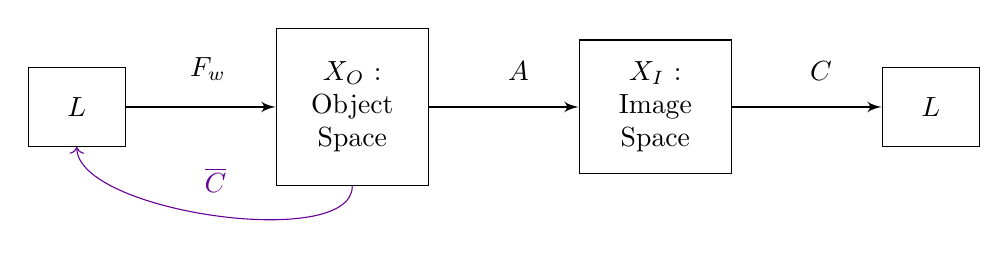
\begin{tikzpicture}%[>=latex,shorten >=2pt,shorten <=2pt,shape aspect=1]

\tikzset{
    connect/.style args={(#1) to (#2) over (#3) by #4}{
        insert path={
            let \p1=($(#1)-(#3)$), \n1={veclen(\x1,\y1)}, 
            \n2={atan2(\y1,\x1)}, \n3={abs(#4)}, \n4={#4>0 ?180:-180}  in 
            (#1) -- ($(#1)!\n1-\n3!(#3)$) 
            arc (\n2:\n2+\n4:\n3) -- (#2)
        }
    },
}

  \node [draw, rectangle, minimum height=1cm, text width = 1cm, text
  centered]
  (fcl) {$L$};
  \node [below=.2cm of fcl] (fclo) {};

  \node [draw, rectangle, minimum height = 2cm , text width = 1.7cm, text
  centered, right = 1.9cm of fcl] (fco) {$X_O$ : Object Space};


  \node [draw, rectangle, draw, minimum height=1.7cm,
   text width = 1.7cm, text centered,
  right = 1.9cm of fco]
  (fci) {$X_I$ : Image Space}; 

  \node [draw, rectangle, draw, minimum height=1cm,
   text width = 1cm, text centered,
  right = 1.9cm of fci]
  (fca) {$L$}; 

  \path [line, thick] (fcl) -- (fcl-|fco.west) node[above left=.2cm and .5cm] {$F_w$};


  \path [line, thick] (fco) -- (fco-|fci.west) node[above left=.2cm and .5cm] {$A$};
  \path [line, thick] (fci) -- (fci-|fca.west) node[above left=.2cm and .5cm] {$C$};
\draw[->,red!40!blue] (fco.south) to[out=-90,in=-90,looseness=.6] (fcl.south) node[above right=-0.7cm and 1.5cm] {$\overline C$};


\end{tikzpicture}
\caption{General Classification: \\
  $F_w$ is a random process producing measures $\mu \in \mathcal M(\R^2)$. \\
  $A : X_O (= \mathcal{M}(\R^2)) \to X_I (= \R^n)$\\
  $C : X_I \to L$ 
}
\label{fig2}
\end{figure}


Type 1: An image whose object measure does not exist under a random
process $F_w$. This may be recognized in the image space if the
manifold of measures is observed in the image space. This manifold
should be of relatively low dimension compared with the dimension of
the image space, and any images that vary in directions orthogonal to
the manifold satisfy Type 1.\\

\vspace{.3cm}

e.g. We can consider the image of the
set of possible handwritten digits under a noiseless
discretization $A$. It is assumed that the image of the manifold $M$ of
handwritten digits in $X_O$, $A(M)$ is low dimensional in $X_I$, thus we can 

\vspace{.3cm}

consider an $\e$-triangulation of this manifold under $A$ with $\e$
the resolution of $A$. A type 1 adversarial image will
be identified as any image that varies more than $\e$ from the
simplices connecting the triangulation of $A(M)$. 

Type 2: A perturbation of an image that is indistinguishable under the
imaging operation (or stochastic imaging process) from an image of an
admissible object.






\section{Computation of a detection algorithm for ``Adversarial''
  examples based on optimal transport}



\url{https://arxiv.org/abs/1801.08926}\\
\url{https://openreview.net/pdf?id=S1EHOsC9tX}\\
\url{http://proceedings.mlr.press/v80/wang18c/wang18c.pdf}\\

\section{Dimensionality reduction on Gaussian samples for slices with
  2 interestnig classes}

better adversarial exmaples. 

apply PCA and plot colored by classification for slices with
exchanging classes.

use NN backpro gradients to identify features (even if not visually)


szegedy and ``deep neural networks are easily fooled'' iccp cvr icml,
adversarial attacks Classification classification neighborhoods of
adversarial examples start with this paper's citations and try to find gaussian (or
other sampling)

\section{Experiment: Gaussian sampling near adversarial images and
  their original images}

We will start with images $I_i^o$ of size 28x28 (MNIST) and adversarial
perturbations generated to shift classification from the original (correct)
classification to each target class $j$  different from the original
$I_{i,j}^a$.   
5000 sample images of noise $I_n$ are  drawn from a Gaussian with
mean 0 
and total variance $\sigma^2$. Due to the nature of sampling high
dimensional Gaussian, $E(|I_n|) = \sigma^2$ i.e. this approximates a
sampling near the surface of a ball with radius $\sigma^2$. \\

Multiple replications of 5000 samples will be generated for $\sigma^2$
ranging from 0 to $\frac{\sigma_a^2}{\sigma_o^2}*40$ -- 40 times the
variance of the adversarial noise divided by the variance of he
original image. (\# TODO update this to pick a consistent range)

\section{Adversarial Attack Lit Review}

The original paper by Szegedy et al. \cite{szegedy2013} is cited 1976 times -- a very extensive body of papers. My goal is to reduce (somewhat) the papers that deserve consideration by looking at more recent works first. I would like to focus on finding the best modern adversarial attack techniques which can be applied to networks trained on MNIST -- specifically those which minimize the noise necessary to perturb classification.

\subsection{FGSM}

Single-step attack tried, need to find something more sophistocated

\subsection{IGSM}

Iterate FGSM to minimize $L_\infty$ norm. (I should definitely try this)

\cite{kurakin_adversarial_2016}

\subsection{L-BFGS minimization of perturbation}
Szegedy et al. set up a box-constrained optimziation problem:

Let $f : \R^m \to \{1,...,k\}$ be a classifier mapping and assume $f$ has an associated continuous loss function denoted by loss$_f : \R^m \times \{1,...,k\} \to \R^+$. \\
\textbf{ Minimize} $\Norm{r}_2$ subject to:
\begin{enumerate}[1.]
\item $f(x + r) = l$
\item $x + r \in [0,1]^m$
\end{enumerate}

Noting that this problem is hard to solve absolutely, they approximate the solution using box-constrained L-BFGS: \\

Find the minimum $c > 0$ for which the minimizer $r$ of the following satisfies $f(x+r) = l$\\

minimize $c|r| + $loss$_f(x+r,l)$ subject to $x + r \in [0,1]^m$.

This technique yields low noise examples, however the adversarial noise is still perceptible on mnist (it should be noted that in their experiments attacking AlexNet, the noise necessary for attacks on higher resolution images was much smaller than on mnist. Presumably the higher dimensionality corresponds with this in some way.


\subsection{Jacobian Based Saliency Map (JSMA)}
\cite{papernot_limitations_2015}
\subsection{Deep Fool (DFool)}
\cite{moosavi-dezfooli_deepfool:_2015}
\subsection{Carlini \& Wagner (C\&W)}
\cite{carlini_towards_2016}


\subsection{Convolutional Network attacked with basic iterative methods}: \url{http://everettsprojects.com/2018/01/30/mnist-adversarial-examples.html}


\section{Generative Adversarial Networks}

\cite{goodfellow2014generative}


\section{Adversarial Conditional Probabilities}

See how activations and output filter determine expected conditional
probabilities under the cross-entropy loss.\\

Plot the activations\\
Plot the filtered outputs

posterior conditional probabilities under

$P(k | X,M)$

Clune's point is we want $P(k) \cdot p(X)$
(Probability of class $k$ times probability of $x$ occuring -- being a
natural image. $p(X)$ is drawn from our distribution function $p(x)$

$x$ is drawn from a pdf describing natural image space.

pdf lives in image space
ideal observer $f'$ and model $f$ have property that $f(X)$,
i.e. $f(p(X))$ is partitioned.

Let $D$ be in object space, $\mathcal{C}$ be our ideal observer, $F$
our observer's writing operation, and $X = F(D)$ in image space.

Then a good classifier has the properties:

\begin{align*}
  0 &\approx P(\mathcal{C}(d) \neq k | C(F(D)) = k)\\
  1 &\approx P(\mathcal{C}(d) = k | C(F(D)) = k)\\
  C_k(X) &= P(\mathcal{C}(d) = k | F(D) = X)\\  
\end{align*}

Want to know $p(x | k)$ the distribution (pdf) of images of class
$k$.

\section{2019-04-03}
advice from Kevin about how to approximate the distribution. 
1-d kolmogorov smirnov compare cdf

\section{Monte-carlo Voting fairness methods to check nn accuracy}

  multi-dimensional fractal dimension of nn classification points.\\

  - can we discriminate noise in the images that beat the test\\
  - define the test in terms of time to decay empirically and see how
  it performs for different adversarial images\\
  - what happens when we try other adversarial examples\\
  - look at the stop sign problem\\
  - define a loss function for the discrimination problem we're
  doing.\\

  Loss\\
  \begin{tabular}{l|l|l|l}
&   $\hat A=0,\hat y=0$ & $A=0,y=1$ & $A=1$\\\hline
    $\hat A=0,\hat y=0$ & 0 & 1 & 10 \\\hline
    $\hat A=0,\hat y=1$ & 1 & 0 & 10 \\\hline
    $\hat A=1,\hat y=0$     & 0.5 & 1 & 0 \\\hline
    $\hat A=1,\hat y=1$     & 1 & 0.5 & 0 \\    
\end{tabular}               

% TODO use torch l-bfgs to generate adversarial examples in pytorch

% generate imagenet classifications with FGSM

%\nocite{*}
\bibliographystyle{abbrv}
%\bibliography{"\string~/Google Drive/UOFA/0-research/bibfile"}
\bibliography{bibfile}
\end{document}

